%%%%%%%%%%%%%%%%%%%%%%%%%%%%%%%%%%%%%%%%%%%%%%%%%%%%%%%%%%%%%%%%%%%%%%
% DelaunayTriangulationSpannerNotes
% March 20th, 2013
% By Simon Pratt (mostly)
\documentclass{tufte-handout}

\usepackage{geometry}
\geometry{verbose,tmargin=1in,bmargin=0.5in,lmargin=.5in}
\usepackage{includes/CGAlgorithms}
\usepackage{includes/TheoremStuff}
\usepackage{includes/HeaderStuff}
\usepackage{natbib}
\usepackage[pdftex]{graphicx}

%%%%%%%%%%%%%%%%%%%%%%%%%%%%%%%%%%%%%%%%%%%%%%%%%%%%%%%%%%%%%%%%%%%%%%
% Configuration
\newcommand{\DocTitle}{Delaunay Graph Spanner Notes}
\newcommand{\DocAuthor}{Simon Pratt}

\title{\DocTitle}
\author{\DocAuthor}
\fancyhead[L]{\DocTitle}
\fancyhead[R]{\DocAuthor}
\bibliographystyle{plain}

%%%%%%%%%%%%%%%%%%%%%%%%%%%%%%%%%%%%%%%%%%%%%%%%%%%%%%%%%%%%%%%%%%%%%%
% Document
\begin{document}

\maketitle
\vspace{1cm}
% Content starts here

In these notes, we discuss the major results with respect to the
Delaunay Graph as a spanner.

\part{Delaunay Graph}

$P$ is a set of points in the plane, $DG(P)$ is a graph whose vertex
set is $P$ where $u$ and $v$ are connected by an edge only if the
voronoi regions for $u$ and $v$ share an edge.

\begin{figure}
  % http://groups.csail.mit.edu/graphics/classes/6.838/F01/lectures/Delaunay/Delaunay2D.ppt
  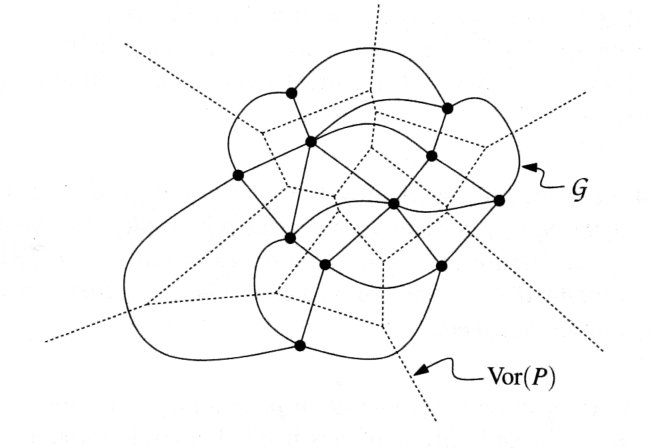
\includegraphics[scale=1.6]{figures/delaunay_graph.png}
  \caption{The Delaunay graph on $P$, including the boundaries of the
    Voronoi regions.}
\end{figure}

\part{Spanner}

Given two points $a,b$ whose euclidean distance from each other is
$d(a,b)$, we would like to prove that a subset of the complete graph
on those points has the property that the distance along the edges in
the path $d_G(a,b)$ is at most $t \cdot d(a,b)$.  Such a graph is
called a $t$-spanner.  We call $t$ the \emph{spanning ratio} of the
spanner.

\newpage

\part{Dobkin's Results}

The Delaunay triangulation of a set of points in the plane is a
spanner with spanning ratio $c \le ((1 + \sqrt{5})/2)\pi \approx
5.08$.  This was proven in the paper ``Delaunay Graphs Are Almost as
Good as Complete Graphs'' by Dobkin, Friedman, and Supowit.  
\cite{Dobkin:1987} \cite{Dobkin:1990}

\section{Introduction}

Let the line segment between $a$ and $b$ be the \emph{direct line}.
We construct \emph{the direct DT path} by following the Delaunay edge
to the representative point each time the direct line crosses into a
new Voronoi region.  Without loss of generality, we can say that the
line segment between points $a$ and $b$ lies on the x-axis.

\begin{Lemma}

  \label{lemma:monotonic:path}

  Points along a direct DT path are monotonic in $x$.

\end{Lemma}

\begin{proof}

  All points along the perpendicular bisector of two adjacent points
  on the direct DT path, $b_i$ and $b_{i+1}$, must be equidistant to
  each of these points.  Since we know these points are adjacent along
  the direct path, they must share a Voronoi edge which must be a
  segment of this bisector.  Since we know the direct line (which is
  the x-axis) crosses this Voronoi edge, we know $b_i$ must lie to the
  left and $b_{i+1}$ must lie to the right of the bisector.
  
\end{proof}

\newpage

\section{One-Sided Path: The Easy Case}

If all edges along the direct DT path between points $a,b \in P$ are
either all above or all below the direct line, we say that this is a
one-sided path.

\begin{figure*}
  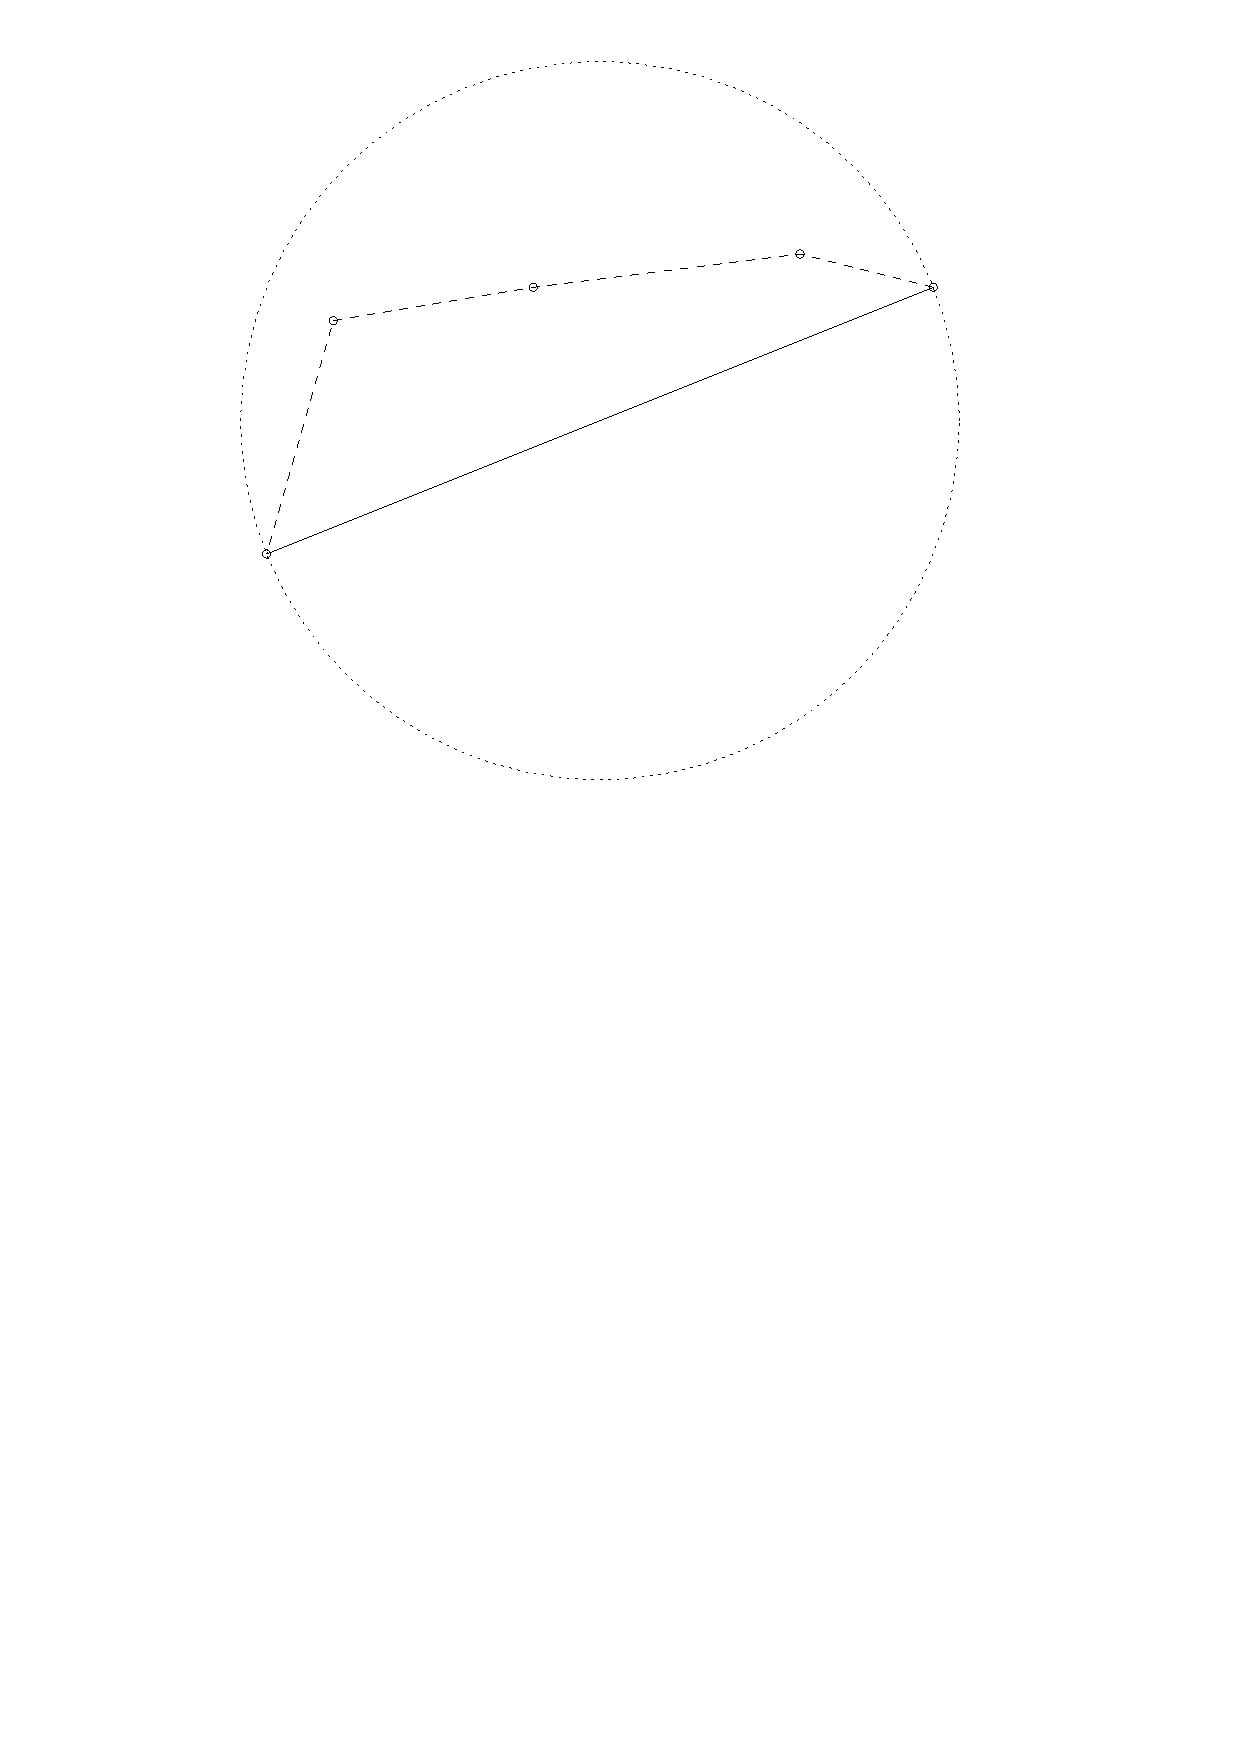
\includegraphics[scale=0.8]{figures/one-sided_path.pdf}
  \caption{The cyan line shows the direct path, the green line shows
    the direct DT path, the dashed red lines show the boundaries of
    the Voronoi regions, and the circumcircles (also dashed) are
    blue.}
\end{figure*}

\begin{Lemma}[3]

  \label{lemma:boundary:circles}

  The boundary of a connected union of $n$ circles centred on a line
  has length at most $\pi \cdot ( x_r - x_l )$ where $x_r$ and $x_l$
  are the extreme x coordinates of any of the circles.
  
\end{Lemma}

\begin{proof}

  We prove by induction that the upper boundary of the circles has
  length at most $\frac{\pi}{2} \cdot ( x_r - x_l )$, from which the
  lemma follows by symmetry.
  
  In the case of a single circle, the upper boundary is half of the
  circumference of the circle:, $\frac{\pi}{2} \cdot ( x_r - x_l )$.
  The lemma holds for $k \ge 1$ circles, we now show that it holds for
  $k+1$ circles.

  Without loss of generality, we say that the $k+1$th circle is added
  at the right-most extremity of the $k$ circles.  

\begin{figure*}
  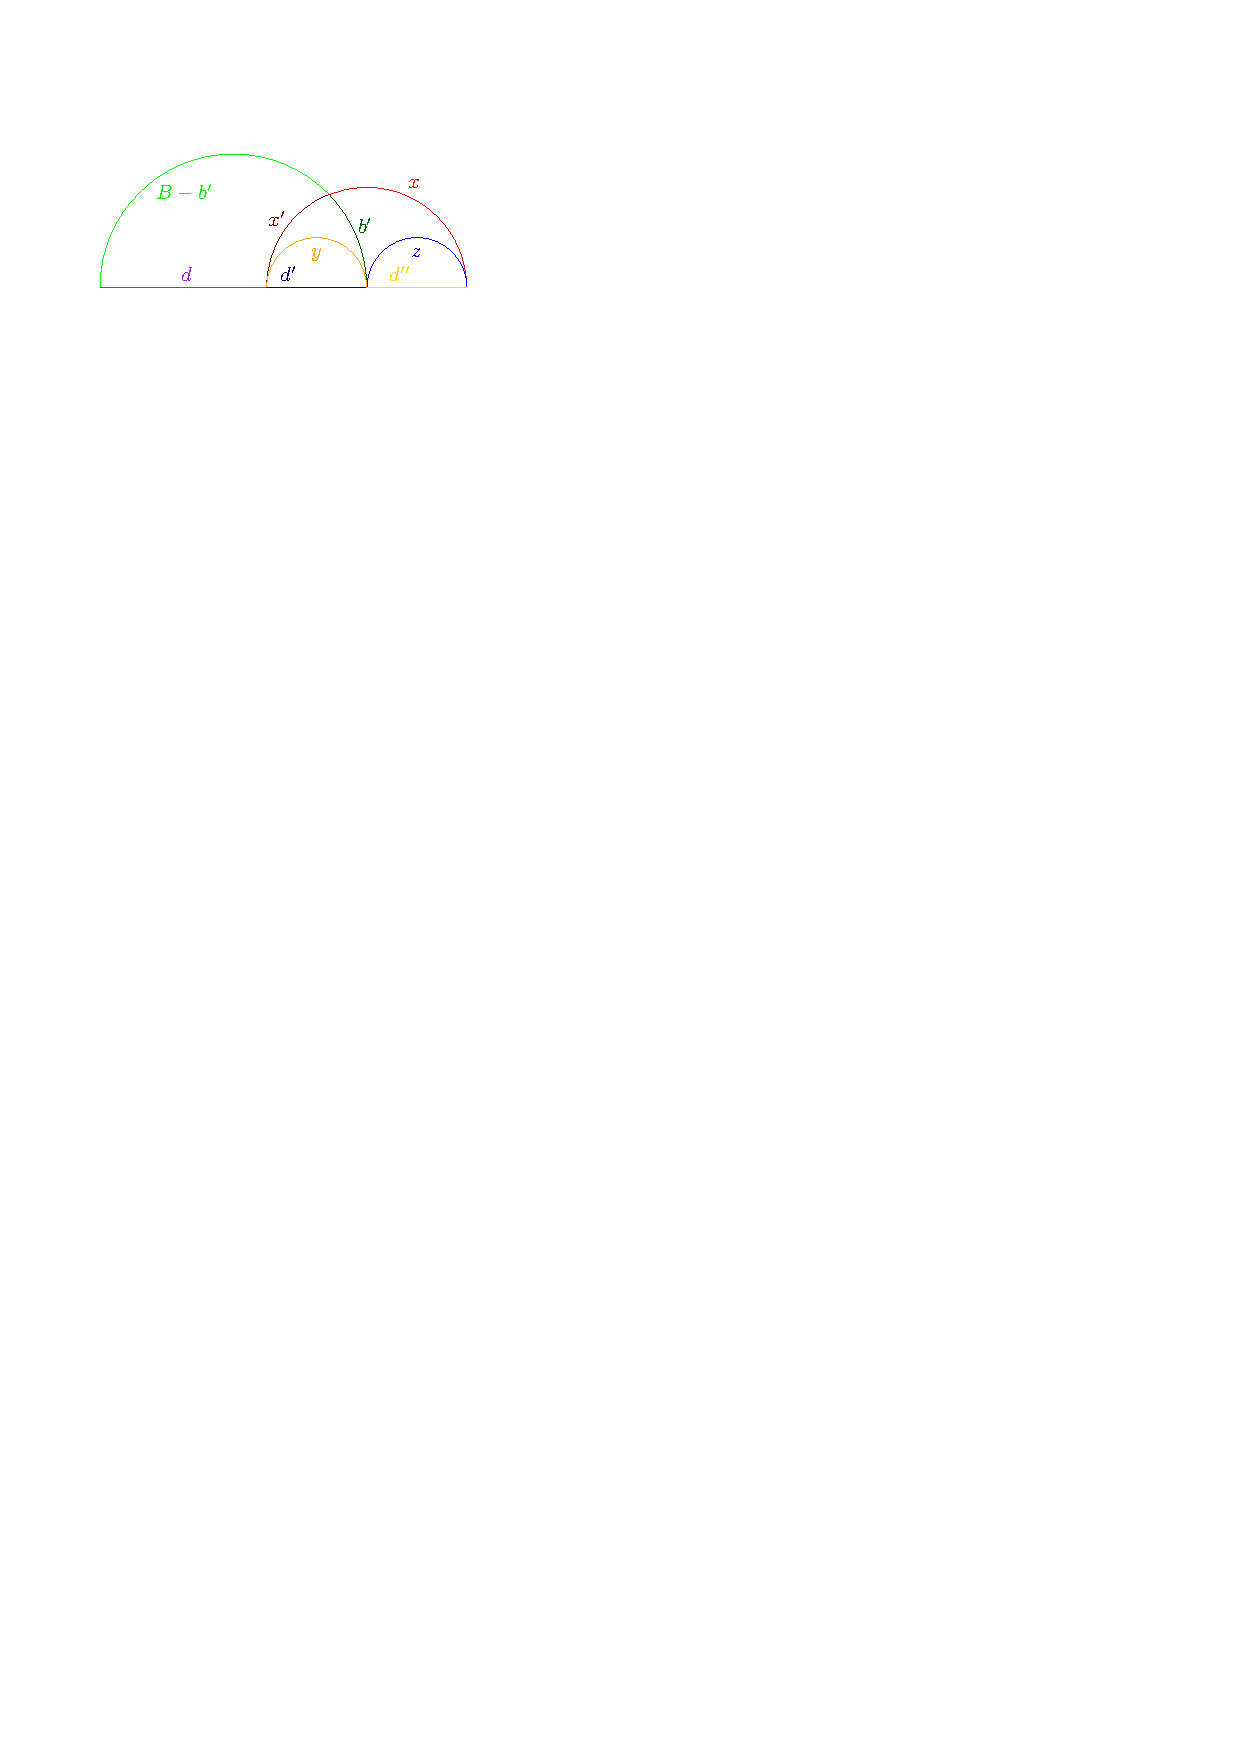
\includegraphics[scale=2.6]{figures/circle_unions.pdf}
  \caption{Let $B$ be the upper boundary of the $k$ circles.  Let $b'$
    be the length of $B$ contained within the $k+1$th circle.  Let $x$
    be the upper boundary of the new circle not contained within $B$,
    and $x'$ be the rest.  Let $y$ be the circle whose left-most point
    is the left-most point of the $k+1$th circle, and whose right-most
    point is the right-most point of $B$.  Let $z$ be the circle whose
    left-most point is the right-most point of $B$ and whose
    right-most point is the right-most point of the $k+1$th circle.}
\end{figure*}

From the inductive hypothesis, we know

\begin{itemize}

\item $B \le \frac{\pi}{2} \cdot (d + d')$

\item $z \le \frac{\pi}{2} \cdot d''$

\end{itemize}

Therefore $B - b' + x \le \frac{\pi}{2} \cdot (d + d' + d'') = B
+ z$.

So we wish to show: $x - b' \le z$.

We know:

\begin{itemize}

\item $y \le x' + b' \leftrightarrow y - x' \le b'$

\item $x' + x = y + z$

\end{itemize}

So

\begin{align*}
  %
  x + x' &= y + z \\
  x &= y + z - x' \\
  x &\le z + b' \\
  x - b' &\le z \\
  %
\end{align*}
  
\end{proof}

Let $a = b_0, \ldots, b_i, \ldots, b_n = b$ be the direct DT path from
$a$ to $b$.  For each pair $b_i, b_{i+1}$ create the circle on whose
boundary these points lie, and whose centre is on the line segment
between $a$ and $b$.  Let the union of these circles be $C$.

From lemma \ref{lemma:boundary:circles}, we know that the length of
the upper half of $C$ is most $\pi/2$ times as long as the euclidean
distance between $a$ and $b$.

From lemma \ref{lemma:monotonic:path}, we know that a one-sided direct
DT path is an x-monotonic path along the upper half of $C$, and
therefore the length of the upper half of $C$ is an upper bound for
the one-sided direct DT path, which is at most $\pi/2$.

\section{The Harder Case}

The direct DT path may cross the x-axis $\BigOmega{n}$ times,
which can yield a much longer path.

\begin{figure}
  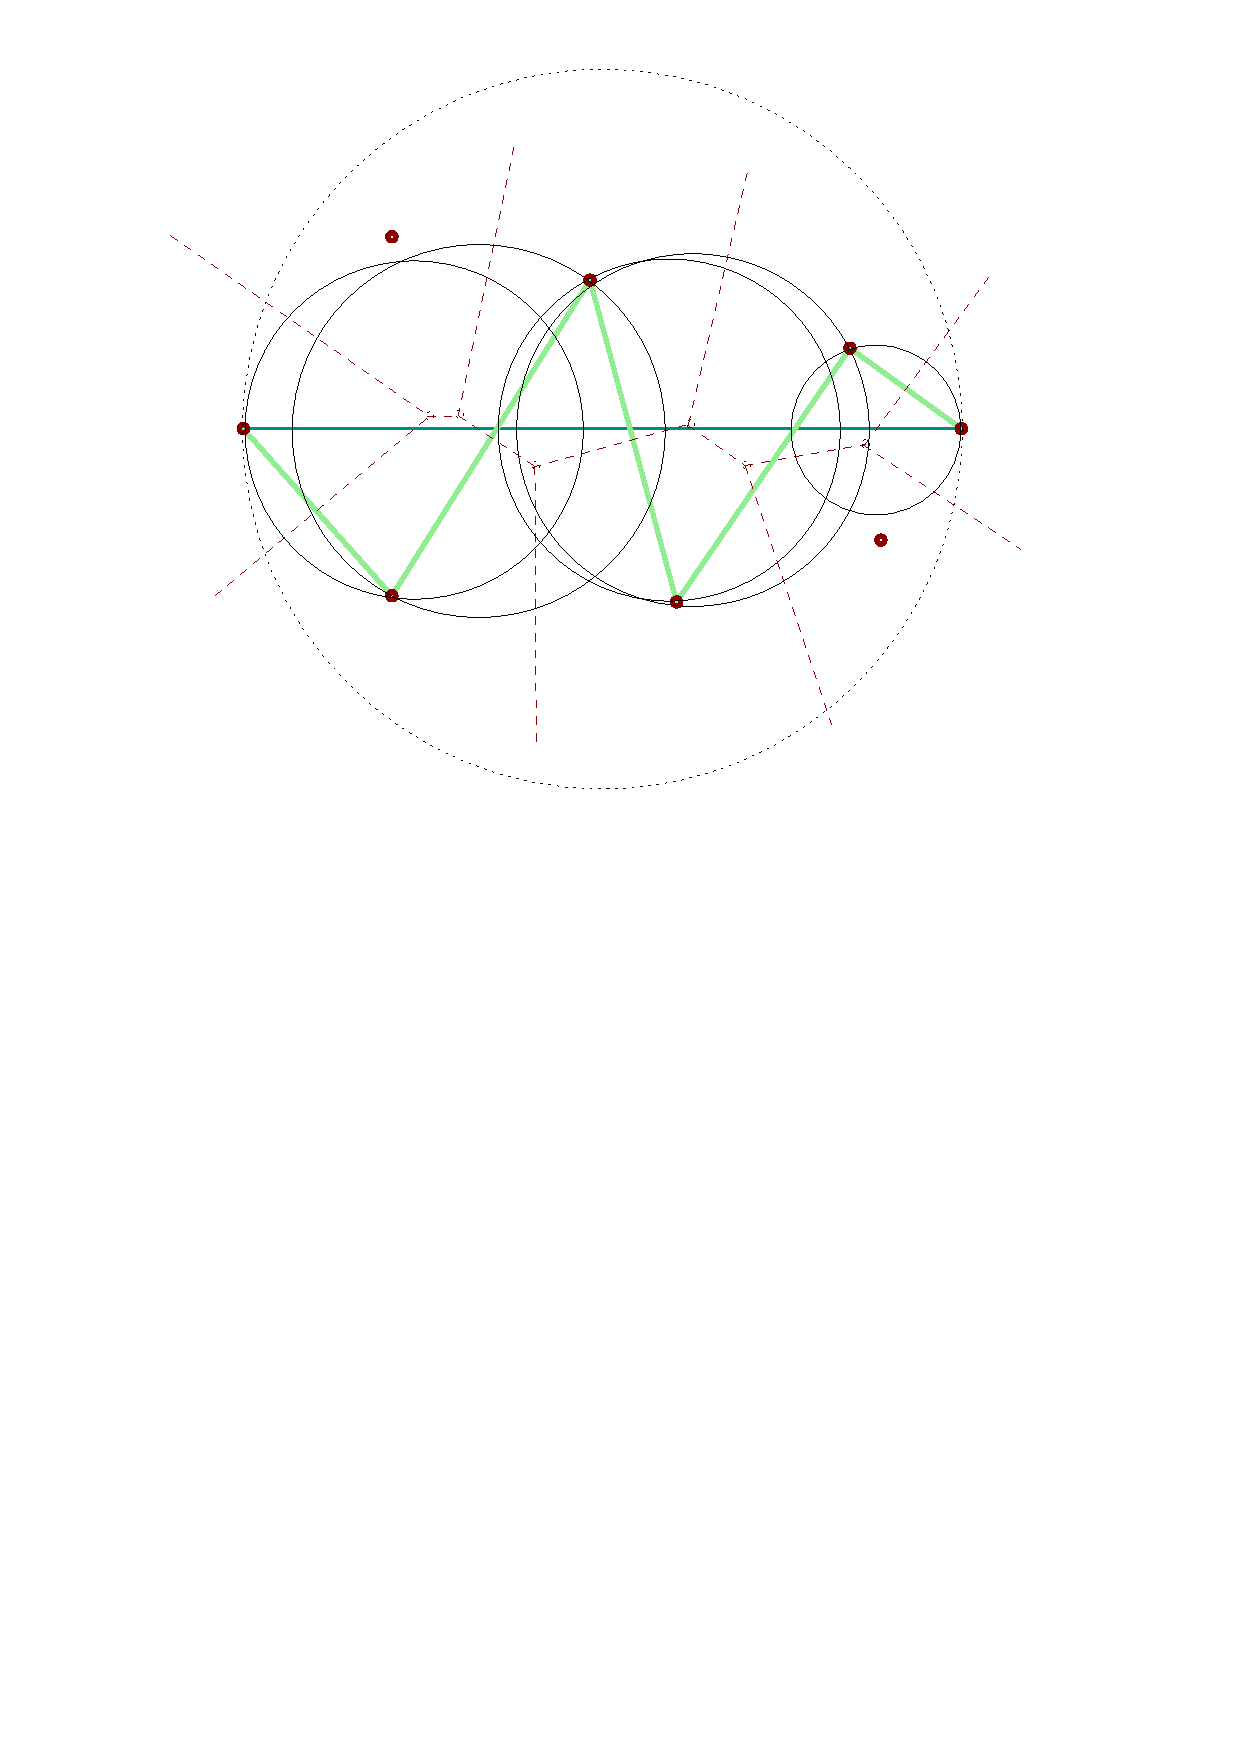
\includegraphics[scale=1.0]{figures/two_sided_path_center_circles.pdf}
  \caption{A two-sided direct DT path showing the circles whose union
    forms $C$ and the dotted circle with $a,b$ diametrically
    opposed.}
\end{figure}

The general idea is that we stick to the region above the x-axis as
much as possible, and follow the path below the x-axis if the distance
travelled across the axis is small compared to the distance travelled
along the path before the next time the path crosses the x-axis.

\begin{figure}
  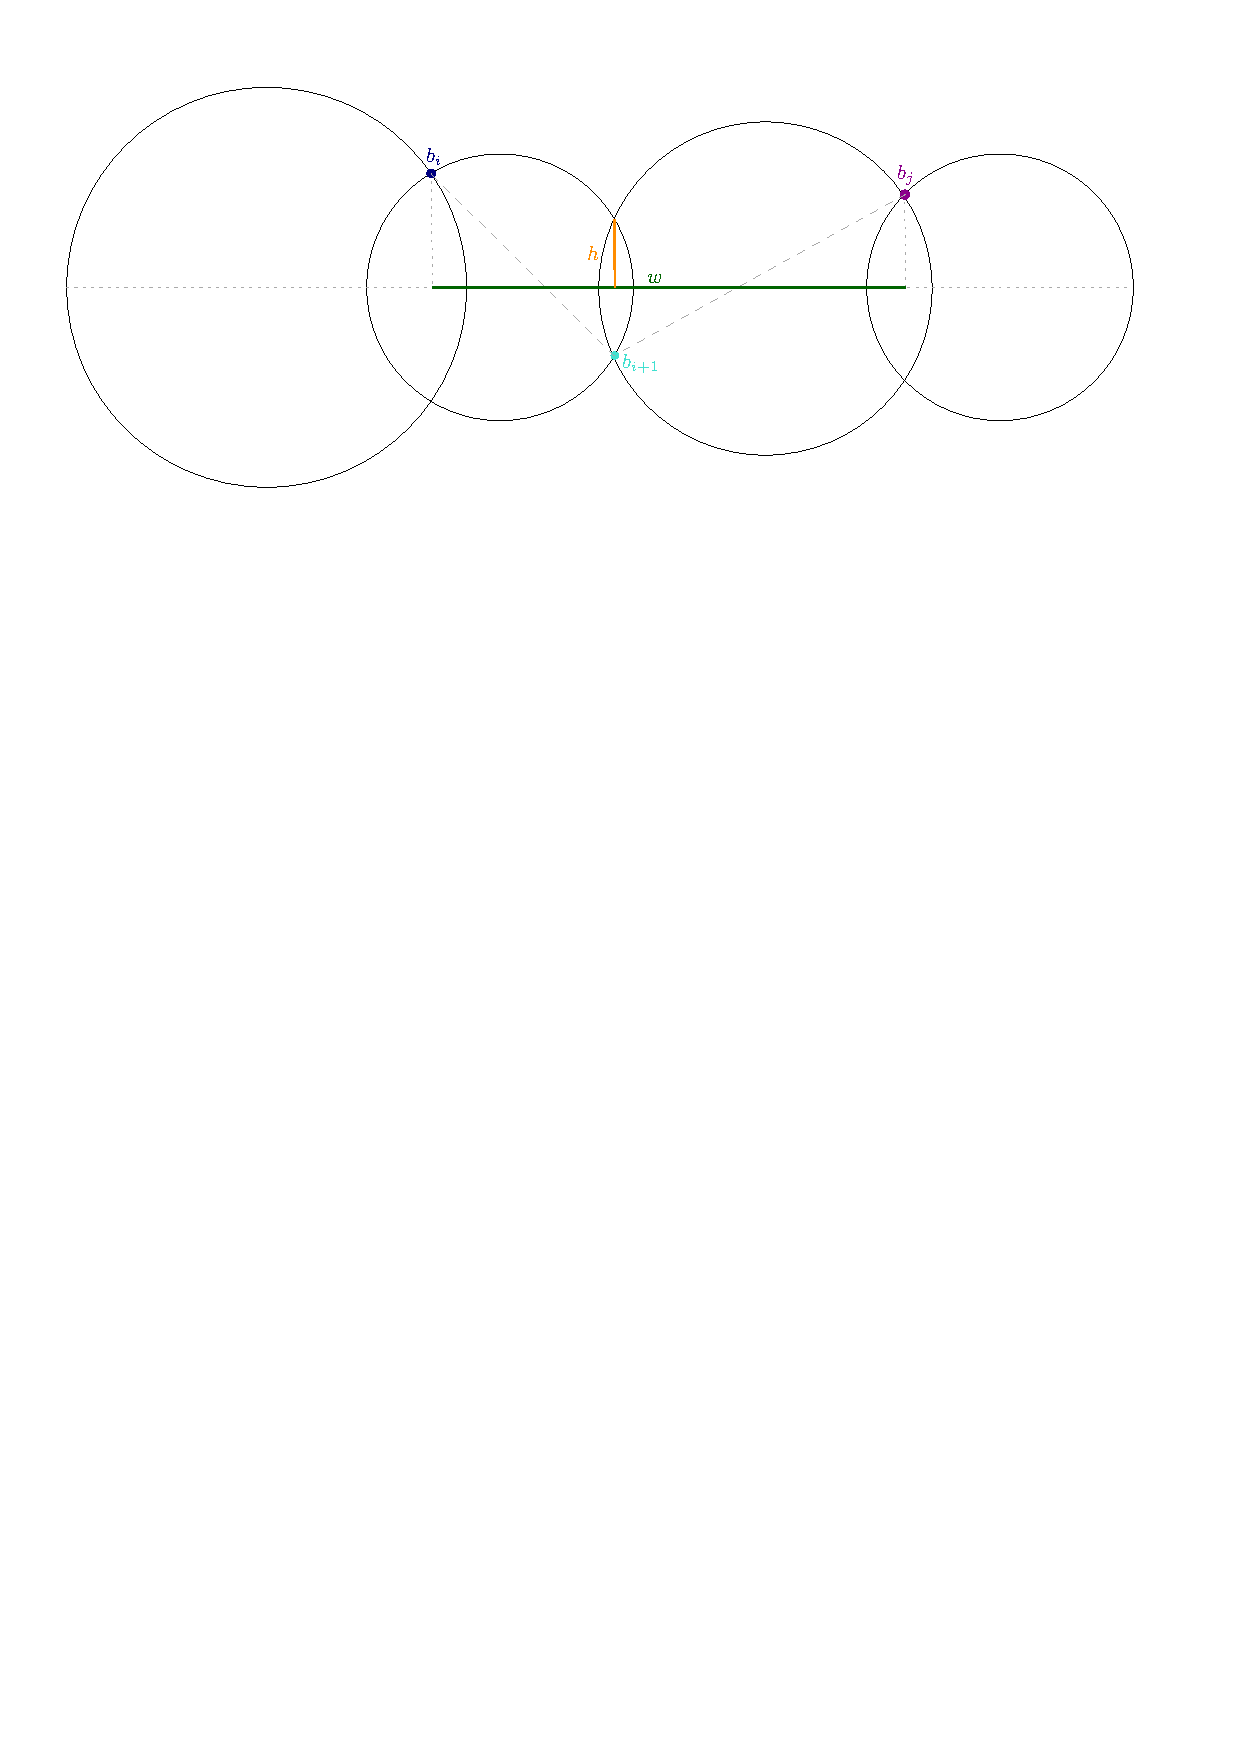
\includegraphics[scale=2.9]{figures/height_width.pdf}

  \caption{
    
    Let $b_i$ be the last point before the direct DT path dips below the
    x-axis, let $b_j$ be the next point after $b_i$ on or above the
    x-axis.  Let $T$ be the section of $C$ between $b_i$ and $b_j$.  Let
    the length of $T$ be $t$.  Let $h = min \{ y(q): q \text{ lies on }
    T \}$, and $w = x(b_j) - x(b_i)$.

    Let $R_1$ be the region between $b_i$ and $b_j$ above the line
    $y=-h$.  Let $R_2$ be the region below the line $y=-h$.  Let $R_3$
    be the region above the line $y=-h$ and to the left of $b_i$.  Let
    $R_4$ be the region above the line $y=-h$ and to the right of
    $b_j$.

  }
\end{figure}

\newpage

To be specific, we take the direct DT path only if $h \le w/4$.

Otherwise, we follow the lower convex hull of all points in $P$
between $b_i$ and $b_j$, who are above the x-axis and below the line
segment between $b_i$ and $b_j$.

The length of the path between $b_i,b_j$ with no shortcuts is at most
$t + 2(y(b_i) + y(b_j))$ and the length of the path between $b_i,b_j$
using the lower hull is at most $t \cdot \pi /2$ (by Lemma 3).

% TODO: add diagram showing lower convex hull

$(z_k,z_{k+1})$ is an edge on the lower convex hull between $b_i$ and
$b_j$.  

\begin{Lemma}[4]

  \label{lemma:convex:path:one:sided}

  The direct DT path from $z_k$ to $z_{k+1}$ is one-sided.
  
\end{Lemma}

Since we know the direct DT path from $z_k$ to $z_{k+1}$ is one-sided,
we know its length is bounded by $\pi/2 \cdot d(z_k,z_{k+1})$.

\begin{Note}
  \label{note:convex:path}

  A convex curve contained within a boundary $B$ has length at most
  the length of $B$. \cite{Benson:1966} % page 42

  % note that I found this reference in Aaron Lee's MCS Thesis

\end{Note}

From note \ref{note:convex:path}, since the lower convex hull is a
convex curve contained within $T$, the sum of the length of all
shortcut edges is at most $\pi/2 \cdot t$.

\newpage

\begin{Note}
  \label{note:right:triangle}

  Where $a,b,c$ are sides of a right triangle with $c$ being the
  hypotenuse, then

  \begin{displaymath}
    %
    \frac{a}{2} + b \le \frac{\sqrt{5}}{2} \cdot c
    %
  \end{displaymath}
  
\end{Note}

\begin{Theorem}

  There exists a DT path from $a$ to $b$ of length

  \begin{displaymath}
    %
    \le \frac{\pi}{2} \cdot (1 + \sqrt{5}) \cdot d(a,b)
    %
  \end{displaymath}

\end{Theorem}

\begin{proof}

  We have shown the shortcut path has length at most $t \cdot \pi /
  2$.

  In the case where $h \le w/4$ and we don't take a shortcut, then let
  $q$ be the lowest point on $T$, $t$ be the length of $T$, $t_i$ be
  the section of $T$ between $b_i$ and $q$, $t_j$ be defined similarly
  for $b_j$, $w_i$ be the projection of $t_i$ on the x-axis, and $w_j$
  be defined similarly for $t_j$.

  The length of the path is at most

  \begin{align*}
    %
    t + 2(y(b_i) + y(b_j)) &= t + 2(2h + (y(b_i) - h) + (y(b_j) - h)) \\
    &\le t + 2(\frac{w}{2} + (y(b_i) - h) + (y(b_j) - h)) \\
    &\le t + 2(\frac{w_i}{2} + (y(b_i) - h) + \frac{w_j}{2} + (y(b_j) - h)) \\
    &\le t + 2(\frac{\sqrt{5}}{2} \cdot t_i + \frac{\sqrt{5}}{2} \cdot t_j)
    \tag{from Note \ref{note:right:triangle}} \\
    &\le t + 2(\frac{\sqrt{5}}{2} \cdot (t_i + t_j)) \\
    &\le t + \sqrt{5} \cdot t \\
    &\le t (1 + \sqrt{5})
    %
  \end{align*}

  From lemma \ref{lemma:boundary:circles}, we know that half the
  boundary of the unioned circles is an upper bound on the length of
  the path, so it must be at most $\frac{\pi}{2} \cdot (1 + \sqrt{5})
  \cdot d(a,b)$.

\end{proof}

\newpage

\section{Secondary Proofs}

Note \ref{note:right:triangle} states if $a,b,c$ are sides of a right
triangle with $c$ being the hypotenuse, then

\begin{displaymath}
  % 
  \frac{a}{2} + b \le \frac{\sqrt{5}}{2} \cdot c
  % 
\end{displaymath}

\begin{proof}[Proof of Note \ref{note:right:triangle}]
  Without loss of generality, assume $b \le a$.
  
  \begin{align*}
    %
    a^2 + b^2 &= c^2 \\
    5a^2 + 5b^2 &= 5c^2 \\
    a^2 + 4a^2 + 5b^2 &= 5c^2 \\
    a^2 + 4a^2 + 4b^2 &\le 5c^2 \\
    a^2 + 4ab + 4b^2 &\le 5c^2 \\
    (a + 2b)^2 &\le 5c^2 \\
    a + 2b &\le \sqrt{5} \cdot c \\
    \frac{a}{2} + b &\le \frac{\sqrt{5}}{2} \cdot c \\
    %
  \end{align*}
\end{proof}

\subsection{Proof of Lemma \ref{lemma:convex:path:one:sided}}

\begin{Lemma}[2]

  \label{lemma:circle:contains:path}

  All points along the direct DT path from $a$ to $b$ are contained
  within or on the boundary of the circle with $a$ and $b$
  diametrically opposed.  \footnotemark
  
\end{Lemma}

% TODO: make this better
  
\begin{proof}
  
  Let $x$ be a point on the direct DT path outside of the circle
  with $a$ and $b$ diametrically opposed, whose centre is $c$.  We
  know $d(x,c) > d(a,c) = d(b,c)$.  Without loss of generality,
  assume $d(a,x) \ge d(b,x)$.  Therefore, $d(a,x) > d(a,c)$.  This
  means the Voronoi region of $x$ could not intersect with the
  direct line between $a$ and $b$.
  
\end{proof}

From Lemma \ref{lemma:circle:contains:path}, we know $circle(z_k,
z_{k+1})$ must contain all the points on the direct DT path from $z_k$
to $z_{k+1}$.  Let the lower half of said circle be $L$.  Without loss
of generality, assume $y(z_k) \le y(z_{k+1})$.

\begin{Note}

  No points of $P$ are within $L$ and $R_3$.
  
\end{Note}

\begin{proof}
  
  From assumption, $L$ and $R_3$ do not intersect.

\end{proof}

\begin{Note}

  No points of $P$ are within $L$ and $R_2$.
  
\end{Note}

\begin{proof}

  Since $z_k \in P$, it must lie above $T$ since it can't be within $C$,
  therefore $y(z_k) \ge h > w/4$ by the fact that we only build this
  lower hull in the case where $h > w/4$.

  TODO: why is $y(q) \le y(z_k)$?

\end{proof}

\begin{Note}

  No points of $P$ are within $L$ and $R_4$.
  
\end{Note}

\begin{proof}

  Any point within $L$ and $R_4$ must also be within $C$.

\end{proof}

Lemma \ref{lemma:convex:path:one:sided} states that the direct DT path
from $z_k$ to $z_{k+1}$ is one-sided.
  
\begin{proof}[Proof of Lemma \ref{lemma:convex:path:one:sided}]

  We prove this by showing that $L$ contains no points of $P$.  From
  Lemmas 4, 5, and 6 it remains only to show that there are no points
  of $P$ within $L$ and $R_1$.

  No points of $P$ in $R_1$ exist between the lines $y=h$ and $y=-h$,
  since this area is strictly within $C$.

  No points of $P$ may exist in $R_1$ above $h$ but below the line
  segment $z_kz_{k+1}$, otherwise it would be on the lower convex hull
  and $z_k$ and $z_{k+1}$ would not be adjacent.

\end{proof}

\newpage
\part{Keil's Results}

TODO

% Content ends here

\newpage

\bibliography{references} % uncomment line to add references

\end{document}
